Given the simulated and measured ABSE spectra (as defined in \secref{sec:04_Auditory_Models:Coloration_Metrics:ABSE}), we first compute the discrepancy, $d_\eta(f_c) = |\eta(f_c) - \eta'(f_c)|$, for each navigation method, source position, microphone spacing, and intermediate microphone position (a total of $1 + (\Delta/0.05)$ distinct positions for each microphone spacing).
We then average, in a single operation, these discrepancies over every combination of microphone spacing and \textit{strictly interior} (i.e., $|u_y| < \Delta/2$) intermediate microphone position (note that this is only $(\Delta/0.05) - 1$ positions per spacing).

\begin{figure}[t]
\centering
  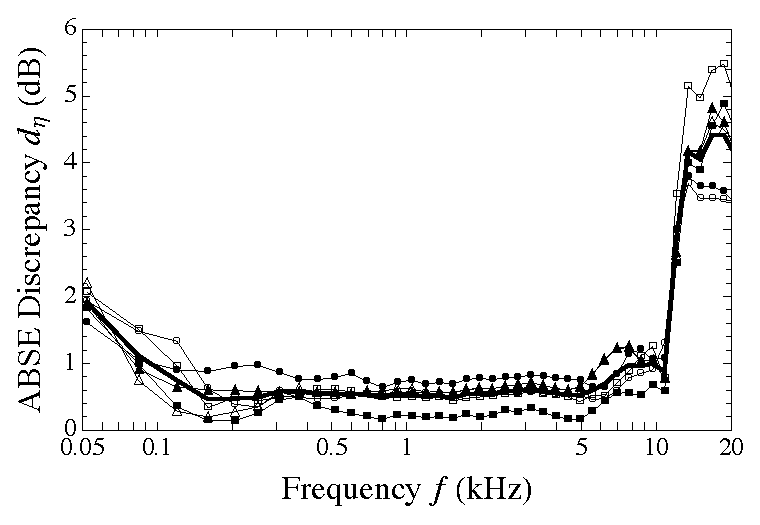
\includegraphics[width = 0.55\textwidth]{10_experimental_validation/figures/scharer2009_fullexp_F.eps}
  \caption[Experimental discrepancies in coloration spectra.]{
  Average discrepancies in ABSE spectra between simulations and measurements.
  Discrepancies are plotted for both the weighted average method (denoted by filled symbols) and the proposed method (empty symbols),
  as well as for each source: A ($\triangle$), B ($\square$), and C ($\bigcirc$).
  For each source and method combination, a thin black line connects the data points, while a thick black line indicates the average over all six curves.}
  \label{fig:10_Experimental_Validation:ABSE_Freq_Discrepancy}
\end{figure}

In \figref{fig:10_Experimental_Validation:ABSE_Freq_Discrepancy}, we plot, as a function of frequency, these average discrepancies in ABSE between the simulations and measurements for each navigation method and source position.
From this plot, we see that the simulations consistently match, within $\sim1$~dB, the physical measurements over a frequency range of approximately $150$~Hz to $10$~kHz.
The sharp increase in discrepancy at high frequencies can be explained by spatial aliasing,
a well-known effect which we do not model in our simulations (see \citet{Rafaely2005a}, for example).
The gradual increase in discrepancy at low frequencies, however, is explained by a combination of a) mismatches between the near-field compensation filters, b) non-anechoic conditions below $\sim425$~Hz, and c) low-frequency ambient noise in the measurements.

\begin{figure}[t]
\centering
  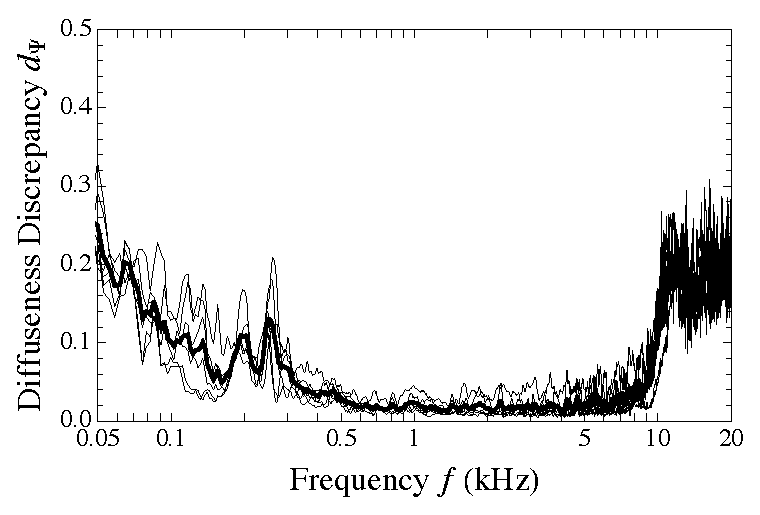
\includegraphics[width = 0.55\textwidth]{10_experimental_validation/figures/merimaa2005_fullexp_F.eps}
  \caption[Experimental discrepancies in diffuseness spectra.]{
  Average discrepancies in diffuseness spectra between simulations and measurements.
  Discrepancies are plotted for both the weighted average method and the proposed method,
  as well as for each source.
  For each source and method combination, a thin black line connects the data points, while a thick black line indicates the average over all six curves.}
  \label{fig:10_Experimental_Validation:Diffuseness_Freq_Discrepancy}
\end{figure}

In \figref{fig:10_Experimental_Validation:Diffuseness_Freq_Discrepancy}, we plot, as a function of frequency, similarly averaged discrepancies in diffuseness (as defined in \secref{sec:04_Auditory_Models:Diffuseness_Parameter}) between the simulations and measurements, given by $d_\Psi(f) = |\Psi(f) - \Psi'(f)|$, for each navigation method and source position.
From this plot, we again see that the simulations consistently match, within $\sim0.1$, the physical measurements over a frequency range of approximately $300$~Hz to $10$~kHz.
Again, spatial aliasing at high frequencies and the other effects mentioned above at low frequencies are evident.

\begin{figure}[t]
    	\centering
    	\begin{subfigure}[b]{0.49\textwidth}
		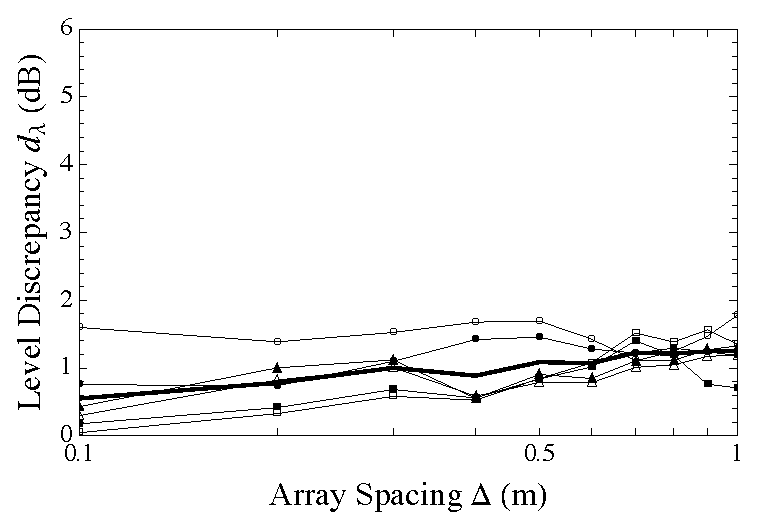
\includegraphics[width=\textwidth]{10_experimental_validation/figures/audibleEnergy_fullexp_D.eps}
		\caption{Level discrepancies}
		\label{fig:10_Experimental_Validation:MAE_Delta_Discrepancy}
    	\end{subfigure}
	\hfill
	\begin{subfigure}[b]{0.49\textwidth}
		\includegraphics[width=\textwidth]{10_experimental_validation/figures/scharer2009_fullexp_D.eps}
		\caption{ABSE discrepancies}
		\label{fig:10_Experimental_Validation:ABSE_Delta_Discrepancy}
    	\end{subfigure}
	
	\vspace{0.5cm}
	\begin{subfigure}[b]{0.49\textwidth}
		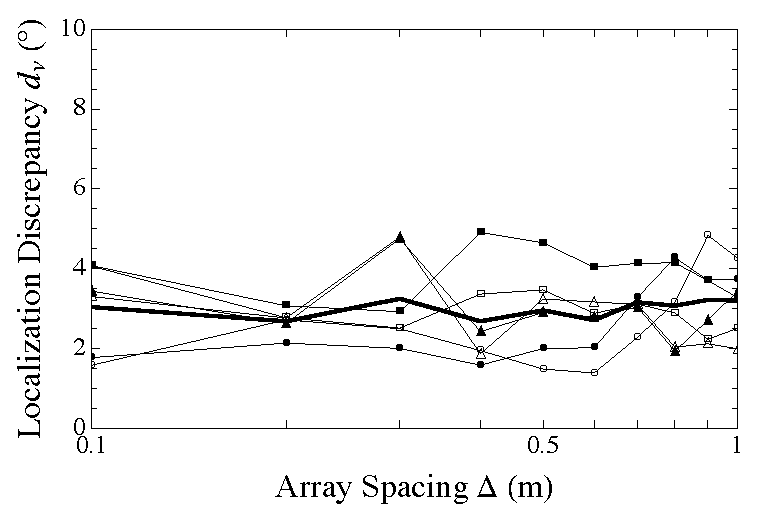
\includegraphics[width=\textwidth]{10_experimental_validation/figures/tylka2017_fullexp_D.eps}
		\caption{Localization discrepancies}
		\label{fig:10_Experimental_Validation:rPE_Delta_Discrepancy}
    	\end{subfigure}
	\hfill
	\begin{subfigure}[b]{0.49\textwidth}
		\includegraphics[width=\textwidth]{10_experimental_validation/figures/merimaa2005_fullexp_D.eps}
		\caption{Diffuseness discrepancies}
		\label{fig:10_Experimental_Validation:Diffuseness_Delta_Discrepancy}
    	\end{subfigure}
	
    	\caption[Experimental discrepancies for each microphone spacing.]{
	Discrepancies in level (top left panel), ABSE (top right), localization direction (bottom left), and diffuseness (bottom right), all plotted for each microphone spacing.
	The ABSE and diffuseness discrepancy spectra were first averaged over $[0,10]$~kHz.
  See \figref{fig:10_Experimental_Validation:ABSE_Freq_Discrepancy} for a description of the lines and symbols used.}
    	\label{fig:10_Experimental_Validation:Delta_Discrepancies}
\end{figure}

In \figref{fig:10_Experimental_Validation:MAE_Delta_Discrepancy}, we plot, now as a function of microphone spacing, the average discrepancies in level (as defined in \secref{sec:04_Auditory_Models:Audible_Energy}), given by $d_\lambda = |\lambda - \lambda'|$, where the average is taken over \textit{all} intermediate microphone positions for each microphone spacing.
From this plot, we see that the level discrepancies are consistently smaller than 2~dB, with a very slight and gradual increase with increasing microphone spacing.

In \figref{fig:10_Experimental_Validation:ABSE_Delta_Discrepancy}, we plot the average discrepancies in ABSE, where two averages are taken: first over all frequencies $f_c \in [0,10]$~kHz and subsequently over all strictly interior intermediate microphone positions.
From this plot we see that the discrepancy between simulation and measurement is consistently smaller than $1$~dB, again with a very slight and gradual increase with increasing microphone spacing.

Given the simulated and measured localization directions (from the localization model described in \secref{sec:05_Proposed_Models:Localization_Model}), we next compute the discrepancy, $d_\nu = \cos^{-1} \left( \hat{\nu} \cdot \hat{\nu}' \right)$, for each navigation method, source position, microphone spacing, and intermediate microphone position.
In \figref{fig:10_Experimental_Validation:rPE_Delta_Discrepancy}, we plot, as a function of microphone spacing, averages of these discrepancies over all strictly interior intermediate microphone positions.
From this plot we see that the discrepancy between simulation and measurement is consistently smaller than $5^\circ$, with an average value of approximately $3.5^\circ$, and does not vary significantly with microphone spacing.

Finally, in \figref{fig:10_Experimental_Validation:Diffuseness_Delta_Discrepancy}, we plot the average discrepancies in diffuseness, where again two averages are taken: first over all frequencies $f \in [0,10]$~kHz and subsequently over all strictly interior intermediate microphone positions.
From this plot we see that the discrepancy between simulation and measurement is consistently smaller than $0.1$ and does not vary significantly with microphone spacing.

Taken together, \figrefthru{fig:10_Experimental_Validation:ABSE_Freq_Discrepancy}{fig:10_Experimental_Validation:Delta_Discrepancies} further suggest that the discrepancies between simulations and measurements do not depend significantly on navigational method or source position.